\chapter{Exercises 5}

\section{Network authentication protocols}

\textbf{\\Q1 - Assume a big company uses a WiFi Access Point (AP) with support for 802.1x and RADIUS for user authentication. 
What is the main role of the AP and what needs to be done to allow it to work when a new EAP method appears?}
\begin{itemize}
    \item[A.] \sol{Allow to perform authentication (through a virtual port) of the users connecting to the AP by encapsulating the EAP messages received from the users (supplicant) into RADIUS messages sent to the AS.}
    \item[C.] Must be updated if new user authentication protocols appear and are supported by EAP.
    \item[D.] \sol{No change is needed if new user authentication protocols appear and are supported by EAP.}
    \item[E.] \sol{Allows to derive session keys (for supplicant and AP) to be used for packet authentication, integrity, and confidentiality.}
\end{itemize}
\com{wip}


\textbf{\\Q2 - Assume a small company uses a WiFi Access Point (AP) enabled with support for 802.1x to authenticate its employees 
when getting access to the corporate network (via a password). What is the main role of the Wi-Fi AP?}
\begin{itemize}
    \item[A.] \sol{Allows to perform authentication of the users connecting to the AP.}
    \item[B.] \sol{Allows to derive session keys (for supplicant and AP) to be used for packet authentication, integrity, and confidentiality.}
    \item[C.] \sol{Allows to perform port-based access control: employees will not get access to the network until they are correctly authenticated.}
\end{itemize}
\com{wip}


\section{Security attacks}

\textbf{\\Q1 - DHCP protocol is subject to attacks because:}
\begin{itemize}
    \item[A.] \sol{The client asking the network configuration is not authenticated.}
    \item[B.] \sol{The client asking the network configuration sends the request in broadcast.}
    \item[C.] The response of the DHCP server is not authenticated.
    \item[D.] The response of the DHCP server is not encrypted.
\end{itemize}
\com{wip}

\textbf{\\Q2 - Assume an attacker knows that a company uses DHCP to provide network configuration. What kind of security attacks can he mount (from the ones explained in the course)?}
\begin{itemize}
    \item[A.] DoS attack (against the DHCP server)
    \item[B.] \sol{DoS attack (against the DHCP client)}
    \item[C.] \sol{MITM attack}
    \item[D.] Replay attack
    \item[E.] Sniffing attack
    \item[F.] \sol{DNS attacks (malicious name-address translation)}
\end{itemize}
\com{wip}


\textbf{\\Q3 - ICMP is a commonly used protocol. What kind of security attacks can be mounted by exploiting its features (from the ones explained in the course)?}
\begin{itemize}
    \item[A.] \sol{Smurfing (by exploiting echo request/reply)}
    \item[B.] \sol{Ping flooding (by exploiting echo request/reply)}
    \item[C.] \sol{MITM attack (by exploiting redirect)}
    \item[D.] Replay attack (by exploiting source quench)
    \item[E.] \sol{DoS attack (by exploiting source quench)}
    \item[F.] MITM attack (by exploiting time exceeded for a datagram)
\end{itemize}
\com{wip}

\textbf{\\Q4 - ARP is a commonly used protocol. ARP poisoning attack is possible because:}
\begin{itemize}
    \item[A.] \sol{the ARP responses are not authenticated}
    \item[B.] \sol{the association between the MAC address to an IP address is changed by the attacker (e.g. by using attack tools)}
    \item[C.] no defense exists against ARP poisoning attack
\end{itemize}
\com{wip}

\textbf{\\Q5 - TCP SYN flooding is a:}
\begin{itemize}
    \item[A.] DoS attack in which the attacker floods the victim with multiple ACK messages in the 3-way TCP handshake so that the victim cannot respond
    \item[B.] \sol{DoS attack in which the attacker sends multiple TCP connection requests with IP source address of a non-existing node, but never sends the ACK}
    \item[C.] \sol{DoS attack which is possible because the victim allocates entries in the TCP connection table when receiving a SYN, and then is waiting for the corresponding ACK}
    \item[D.] an attack against which it is very difficult to defend from
\end{itemize}
\com{wip}

\textbf{\\Q6 - Indicate (some of the) possible attacks against DNS:}
\begin{itemize}
    \item[A.] \sol{DNS shadow server}
    \item[B.] \sol{DNS cache poisoning (affecting the local NS)}
    \item[C.] \sol{wrong configuration of the resolver on the (DNS) client}
    \item[D.] \sol{data corruption (on the victim node) or on the zone files}
    \item[E.] replay of DNS requests
    \item[F.] capture sensitive information from the DNS responses
    \item[G.] \sol{user privacy problems for the queries}
\end{itemize}
\com{wip}


\section{IPsec and VPN}

\textbf{\\Q1- A VPN is:}
\begin{itemize}
    \item[A.] \sol{a technique to create a private network, typically uniting physically distant users or subnetworks through cryptographic protection of the network packets (secure IP tunnel)}
    \item[B.] \sol{a technique to create a private network, typically uniting physically distant users or subnetworks through the use of techniques such as:
    \begin{itemize}
        \item private addressing,
        \item protected routing (IP tunnel), or
        \item via cryptographic protection of the network packets (secure IP tunnel)
    \end{itemize}}
\end{itemize}
\com{wip}

\textbf{\\Q2 - assume that two companies (Oil Torino, and Food Melfi)
decide to create a VPN via private IP addresses.}
\begin{figure}[h]
    \centering
    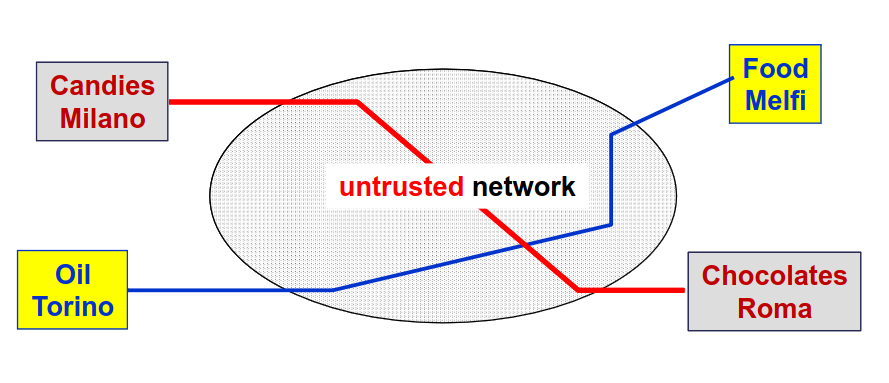
\includegraphics[width = 0.70\textwidth]{exercises5/question2.png}
\end{figure}
\textbf{Which kind of attacks can be mounted by an attacker?}
\begin{itemize}
    \item[A.] \sol{Assume an attacker in the network: inject fake packets by guessing or discovering the IP addresses used by the two companies}
    \item[B.] \sol{Assume an attacker in the network: sniff the packets during transmission over the shared channels}
    \item[C.] \sol{Assume an attacker inside the telecom operator: get unauthorized access to the communication devices (routers) to intercept the transmission, replay, or inject new packets}
    \item[D.] \sol{Assume an attacker (inside the telecom operator or in the network): the DoS attack}
\end{itemize}
\com{wip}


\textbf{\\Q3 - Assume two companies (Oil Torino and Food Melfi) decide to create a VPN via IP tunnel (IP in IP).
Other two companies (Candies Milano and Chocolates Roma) also decide to create a VPN via IP tunnel (IP in IP).}
\begin{figure}[h]
    \centering
    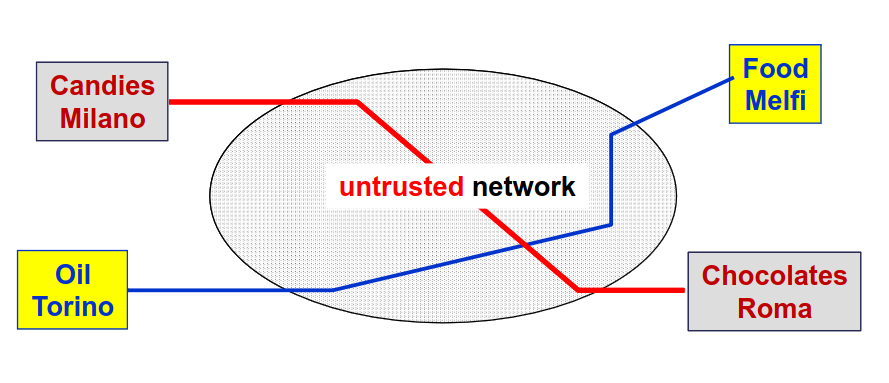
\includegraphics[width = 0.70\textwidth]{exercises5/question2.png}
\end{figure}
\textbf{Which kind of attacks can be mounted by an attacker?}
\begin{itemize}
    \item[A.] Assume an attacker inside Candies Milano: he can inject fake packets by guessing or discovering the addresses used by Oil Torino
    \item[B.] \sol{Assume an attacker in the network: he can sniff (read the content of) the packets during transmission over the shared channels}
    \item[C.] \sol{Assume an attacker inside the telecom operator: if he can get unauthorized access to the communication devices (routers), then he can intercept the packets, replay, or inject new packets}
    \item[D.] \sol{Assume an attacker (inside the telecom operator or in the network): he can perform the DoS attack}
\end{itemize}
\com{wip}


\textbf{\\Q4 - Assume two companies (Candies Milano and Chocolates Roma) decide to create a VPN via secure IP tunnel}
\begin{figure}[h]
    \centering
    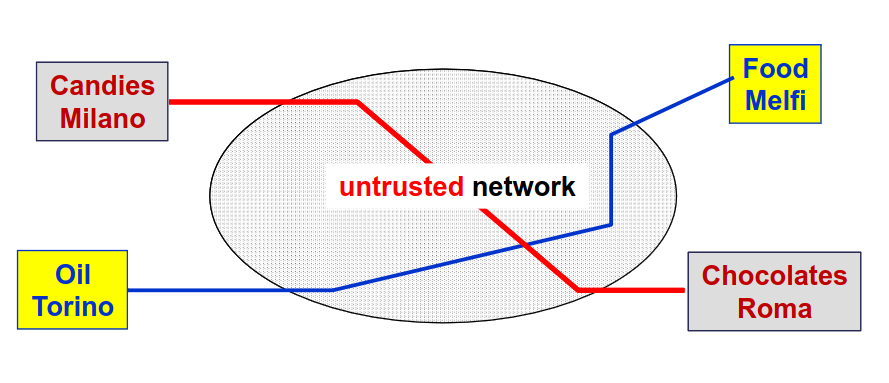
\includegraphics[width = 0.70\textwidth]{exercises5/question2.png}
\end{figure}
\textbf{Which kind of attacks can be mounted by an attacker?}
\begin{itemize}
    \item[A.] An attacker inside Candies Milano: he can inject fake packets by guessing or discovering the addresses used by Oil Torino
    \item[B.] An attacker in the network: he can sniff (read the content of) the packets during transmission over the shared channels
    \item[C.] An attacker inside the telecom operator: if he can get unauthorized access to the communication devices (routers), then he can intercept the packets, replay, or inject new packets
    \item[D.] \sol{An attacker (inside the telecom operator or in the network): he can perform the DoS attack}
\end{itemize}
\com{wip}

\textbf{\\Q5 - The IPsec protocol provides security services:}
\begin{itemize}
    \item[A.] At application level
    \item[B.] At transport level
    \item[C.] \sol{At network level}
    \item[D.] At data link level
\end{itemize}
\com{wip}

\textbf{\\Q6 - The SPD in IPsec contains:}
\begin{itemize}
    \item[A.] List of active algorithms, keys, parameters to apply for the protection of the IP packets
    \item[B.] \sol{List of rules that may depend on fields in the IP and transport-layer headers (e.g., destination address and port, source address and port, protocol) indicating whether IPsec needs to be applied to the packet}
\end{itemize}
\com{wip}

\textbf{\\Q7 - A company decides to adopt end-to-end security to protect communication between its end nodes. Moreover, it decides each node must protect the IP packets both with AH and ESP. Assume two nodes A and B. Consider the node A: how many SAs and SPs does it need to configure in the IPsec module to communicate with the node B?}
\begin{itemize}
    \item[A.] One SA and one SP
    \item[B.] Two SAs and one SP
    \item[C.] Two SAs and two SPs
    \item[D.] \sol{Four SAs and two SPs}
\end{itemize}
\com{wip}

\textbf{\\Q8 - Assume a company decides to adopt end-to-end security IPsec schema between all its nodes (placed at different locations). 
Which steps must be fulfilled to accomplish this task and which are the possible drawbacks?}
\begin{itemize}
    \item[A.] \sol{Install (and configure) IPsec on all the nodes}
    \item[B.] \sol{In case ESP (with confidentiality) is used, then (internal) network monitoring, filtering of traffic based on the content, as well IDS will not be possible}
    \item[C.] Install (and configure) IPsec only on the gateway
    \item[D.] \sol{In case ESP is used, the IP header (original) is not protected when transmitted over the untrusted network}
    \item[E.] \sol{Possible performance problems can be encountered at some hosts (e.g. ones acting as servers) due to IPsec load}
\end{itemize}
\com{wip}

\textbf{\\Q9 - Assume a company decides to adopt Basic VPN IPsec schema between all its nodes (placed at different locations). 
Which steps must be fulfilled to accomplish this task and which are the possible drawbacks?}
\begin{itemize}
    \item[A.] Install (and configure) IPsec on all the nodes
    \item[B.] In case ESP (with confidentiality) is used, then (internal) network monitoring, filtering of traffic based on the content, as well IDS will not be possible
    \item[C.] \sol{Install (and configure) IPsec only on the gateway}
    \item[D.] In case ESP is used, the IP header (tunnel) is not protected when transmitted over the untrusted network
    \item[E.] \sol{Possible performance problems can be encountered at the gateway due to IPsec load}
\end{itemize}
\com{wip}

\textbf{\\Q10 - The (partial) protection against replay in IPsec is performed}
\begin{itemize}
    \item[A.] By a sequence number, inserted in the IP packet
    \item[B.] \sol{By a sequence number, inserted in the AH or ESP headers}
    \item[C.] By counting how many packets have been received and confronting the number against a specific field in the AH or ESP headers
    \item[D.] \sol{By exploiting a moving window (packets received that are outside the window are dropped)}
    \item[E.] By exploiting a moving window (packets received that are outside the window are accepted)
\end{itemize}
\com{wip}

\textbf{\\Q11a - What is IKE in IPsec?}
\begin{itemize}
    \item[A.] An important component in IPsec that automates key establishment by using RSA
    \item[B.] \sol{A combination of a protocol needed to negotiate, set-up, modify and delete a SA (ISAKMP) and a protocol for authenticated key exchange of symmetric keys (OAKLEY)}
\end{itemize}
\textbf{\\Q11b - How IKE supports the negotiation of SAs?}
\begin{itemize}
    \item[A.] \sol{It creates first a SA to protect the ISAKMP exchange; then this SA is used to protect the negotiation of the SA needed by IPsec traffic.}
    \item[B.] It creates directly a SA used to protect the IPsec traffic.
\end{itemize}
\com{wip}

\section{Firewalls}

\textbf{\\Q1 - Which are the design goals of a (network) firewall?}
\begin{itemize}
    \item[A.] \sol{Only the 'authorized' traffic can traverse the firewall.}
    \item[B.] The firewall must detect traffic that does not satisfy specific rules and raise alarms.
    \item[C.] \sol{The firewall must be a highly secure system itself.}
    \item[D.] The firewall is a special-purpose device which allows creating secure tunnels with the internal trusted nodes.
    \item[E.] \sol{The firewall must be the only contact point between the internal network and the external one.}
\end{itemize}

\textbf{\\Q2 - Assume a company decides to adopt the default-deny (also known as allowlist) authorization policy for its firewall configuration. What does it mean?}
\begin{itemize}
    \item[A.] \sol{By default, every network service is denied.}
    \item[B.] By default, every network service is allowed.
    \item[C.] \sol{The administrator must create a list of few known services and configure the firewall to allow access only to those services.}
    \item[D.] The administrator must create a list of potentially dangerous services and configure the firewall to block access for those services.
\end{itemize}

\textbf{\\Q3 - Assume a company decides to adopt a packet filter (as a firewall) placed at the border router between the external network and the internal one. What does it mean?}
\begin{itemize}
    \item[A.] \sol{The administrator must create a list of rules containing (typically) source IP address, source port number, destination IP address, destination port number, protocol (e.g., tcp, udp), and the action to be performed on the packet (allow, drop).}
    \item[B.] The administrator must install a specific filter on the router, one for each application (e.g., FTP, SMTP, HTTP, TELNET).
    \item[C.] The administrator may easily block attacks originating from traced IP addresses.
    \item[D.] The internal nodes are well protected from external attacks (e.g., TCP SYN flooding or ping bombing).
\end{itemize}

\textbf{\\Q4 - Assume a company decides to adopt a ‘dual-homed gateway’ architecture to protect access to his web server (placed on the internal network). What does it mean?}
\begin{itemize}
    \item[A.] \sol{The administrator must create a list of rules for the packet filter containing (typically) source IP address, source port number, destination IP address, destination port number, protocol, and the action (allow, drop) to be performed on the packet.}
    \item[B.] \sol{The administrator must install a specific application filter on the gateway for the web traffic (HTTP/S).}
    \item[C.] \sol{If the web server has a bug, the internal nodes are protected anyway.}
    \item[D.] \sol{The administrator must configure two (filtering) systems instead of one.}
\end{itemize}

\textbf{\\Q5 - Assume a company decides to adopt a ‘screened host’ architecture to protect access to his web server (placed on the same subnetwork of the gateway). What does it mean?}
\begin{itemize}
    \item[A.] \sol{The administrator must create a list of rules for the packet filter containing (typically) source IP address, source port number, destination IP address, destination port number, protocol, and the action (allow, drop) to be performed on the packet.}
    \item[B.] \sol{The administrator must install a specific application filter on the gateway for the web traffic (HTTP/S).}
    \item[C.] If the packet filter has a bug, the internal nodes are protected anyway.
    \item[D.] \sol{The administrator must configure two (filtering) systems instead of one.}
\end{itemize}

\textbf{\\Q6 - Assume a company decides to adopt a ‘screened subnet’ architecture to protect access to its web server (placed on the same subnetwork as the gateway). What does it mean?}
\begin{itemize}
    \item[A.] \sol{The administrator must create a list of rules for two packet filters, possibly from different vendors, containing (typically) source and destination IP addresses and port numbers, protocol, and the action (allow, drop) to be performed on the packets.}
    \item[B.] \sol{The administrator must install a specific application filter on the gateway for the web traffic (HTTP/S).}
    \item[C.] If one packet filter has a bug, the internal nodes are protected anyway.
    \item[D.] \sol{The administrator must configure two (filtering) systems instead of one.}
\end{itemize}
